% !TEX root = base.tex 

\chapter{Hematite Reactivity on Single Crystal Substrates}
\label{ch:single.crystal.reactivity}


\chintro{The majority of the text in this chapter appears in \emph{Chemical
Communications}, 2012, 48 (14), 2012-2014.\cite{Schultz:2012cr} This chapter describes the
reactivity of thin films of \textalpha-\ce{Fe2O3} on various single crystal substrates.
The key discovery reported in this section is that thin films of \textalpha-\ce{Fe2O3}
show drastically differing levels of photochemical reactivity when supported on different
substrates. (0001)-oriented \ce{Fe2O3} on (111)-oriented \ce{SrTiO3} substrates are
significantly more reactive than films supported on (0001)-\ce{Al2O3} or even bulk
polycrystalline \ce{Fe2O3}. Previous work in the \ce{SrTiO3}/\ce{Fe2O3} system has focused 
on improving the activity of \ce{SrTiO3} through the incorporation of \ce{Fe2O3} as an electron
scavenger.\cite{Luo:2006kg,Wang:2007fp} Those experiments tested the activity of the
heterostructures towards photochemical oxidation (with \ce{SrTiO3} acting as a
photoanode). Here, the behavior of \ce{Fe2O3}/\ce{SrTiO3} heterostructures is tested in
the reverse configuration. \ce{Fe2O3} is the active material, supported on \ce{SrTiO3},
and acts as a photocathode for reducing aqueous \ce{Ag+} to solid Ag.}
 
 
\section{Experimental Details}
\label{sec:single.crystal.experimental}

 
\ce{Fe2O3} films were deposited on various substrates using pulsed laser deposition. Basic
procedures outlined in Chapter~\ref{ch:experimental} were followed for pulsed laser
deposition and synthesis of a polycrystalline hematite target. Films were deposited on
single crystal \ce{SrTiO3} (111) and \ce{Al2O3} (0001) substrates. Both films were
verified as (0001) oriented via X-ray diffraction. Bulk \ce{Fe2O3} was prepared as
described in \S \ref{subsec:exp.solidstate}.


\section{Results}
\label{sec:single.crystal.results}


\figureref{thinfilmresults} shows \abbr{AFM} images of the film surfaces before and after
reaction with the AgNO3 solution.  
\begin{figure}
	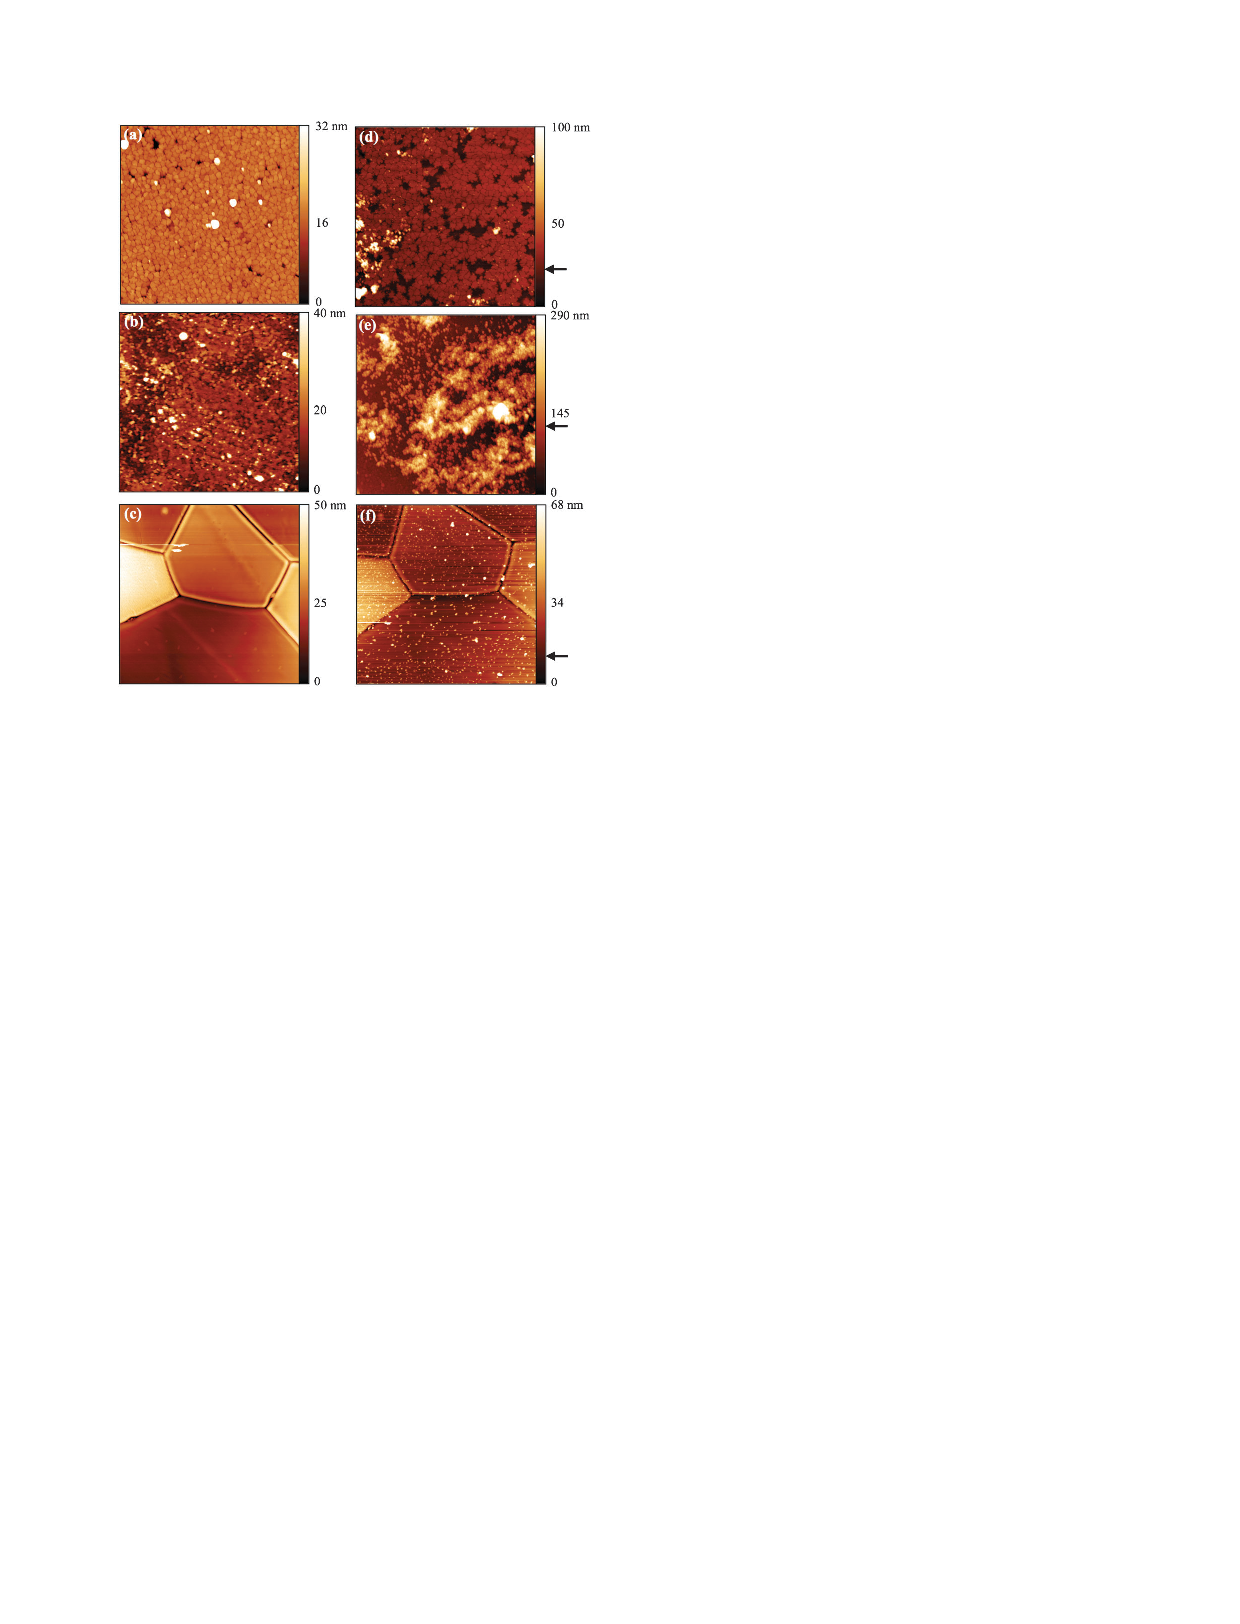
\includegraphics[width=\textwidth]{thinfilmresults.pdf}
	\caption[Images of thin film surfaces after reaction]{%
		Topographic \abbr{AFM} images of sample surfaces before (a-c) and 
		after (d-f) the photochemical reduction of Ag from an aqueous 
		\ce{AgNO3} solution. (a) and (d) show the surface of the 
		\ce{Fe2O3} film supported on \ce{Al2O3}, (b) and (e) show 
		the \ce{Fe2O3} film on \ce{SrTiO3}, and (c) and (f) show bulk 
		polycrystalline \ce{Fe2O3}. The arrows next to the micrographs 
		in (d-f) indicate the location of the horizontal line used for 
		\figureref{lineprofiles}.}
	\label{fig:thinfilmresults}
\end{figure}
\figureref{thinfilmresults}(a) and \figureref{thinfilmresults}(b) show the clean surface
of the \ce{Fe2O3} films on \ce{SrTiO3} and \ce{Al2O3}, respectively. 
\figureref{thinfilmresults}(c) shows the clean surface of bulk \ce{Fe2O3}. The
corresponding surfaces after reaction are shown in Figures
\figureref{thinfilmresults}(c)-(e). All areas are \SI{10}{\micro\meter} x
\SI{10}{\micro\meter}, but the vertical scales differ. After reaction, the surface of the
film on alumina, \figureref{thinfilmresults}(d), shows occasional small silver deposits,
visible as bright spots on the micrograph.  The surface of the film on the
\ce{SrTiO3}(111) substrate, shown in \figureref{thinfilmresults}(e), is covered in a
thick, inhomogeneous layer of reaction product.  The amount of silver present after
reaction on the film supported on the \ce{SrTiO3} substrate is much greater than for the
film on alumina or for the bulk sample in \figureref{thinfilmresults}(f).  Of particular
note is the difference in vertical scales for the micrographs after the photochemical
reduction of Ag.  The vertical scale for the reaction on the \ce{SrTiO3} supported film is
\SI{290}{\nano\meter}, as compared to \SI{100}{\nano\meter} and \SI{68}{\nano\meter} for
the film on alumina and the bulk hematite, respectively. The (0001) oriented film on
\ce{SrTiO3} is significantly more reactive than the (0001) grains observed for bulk
\ce{Fe2O3}, reported in \chapterref{fe2o3orientation}.

\begin{figure}
\begin{center}
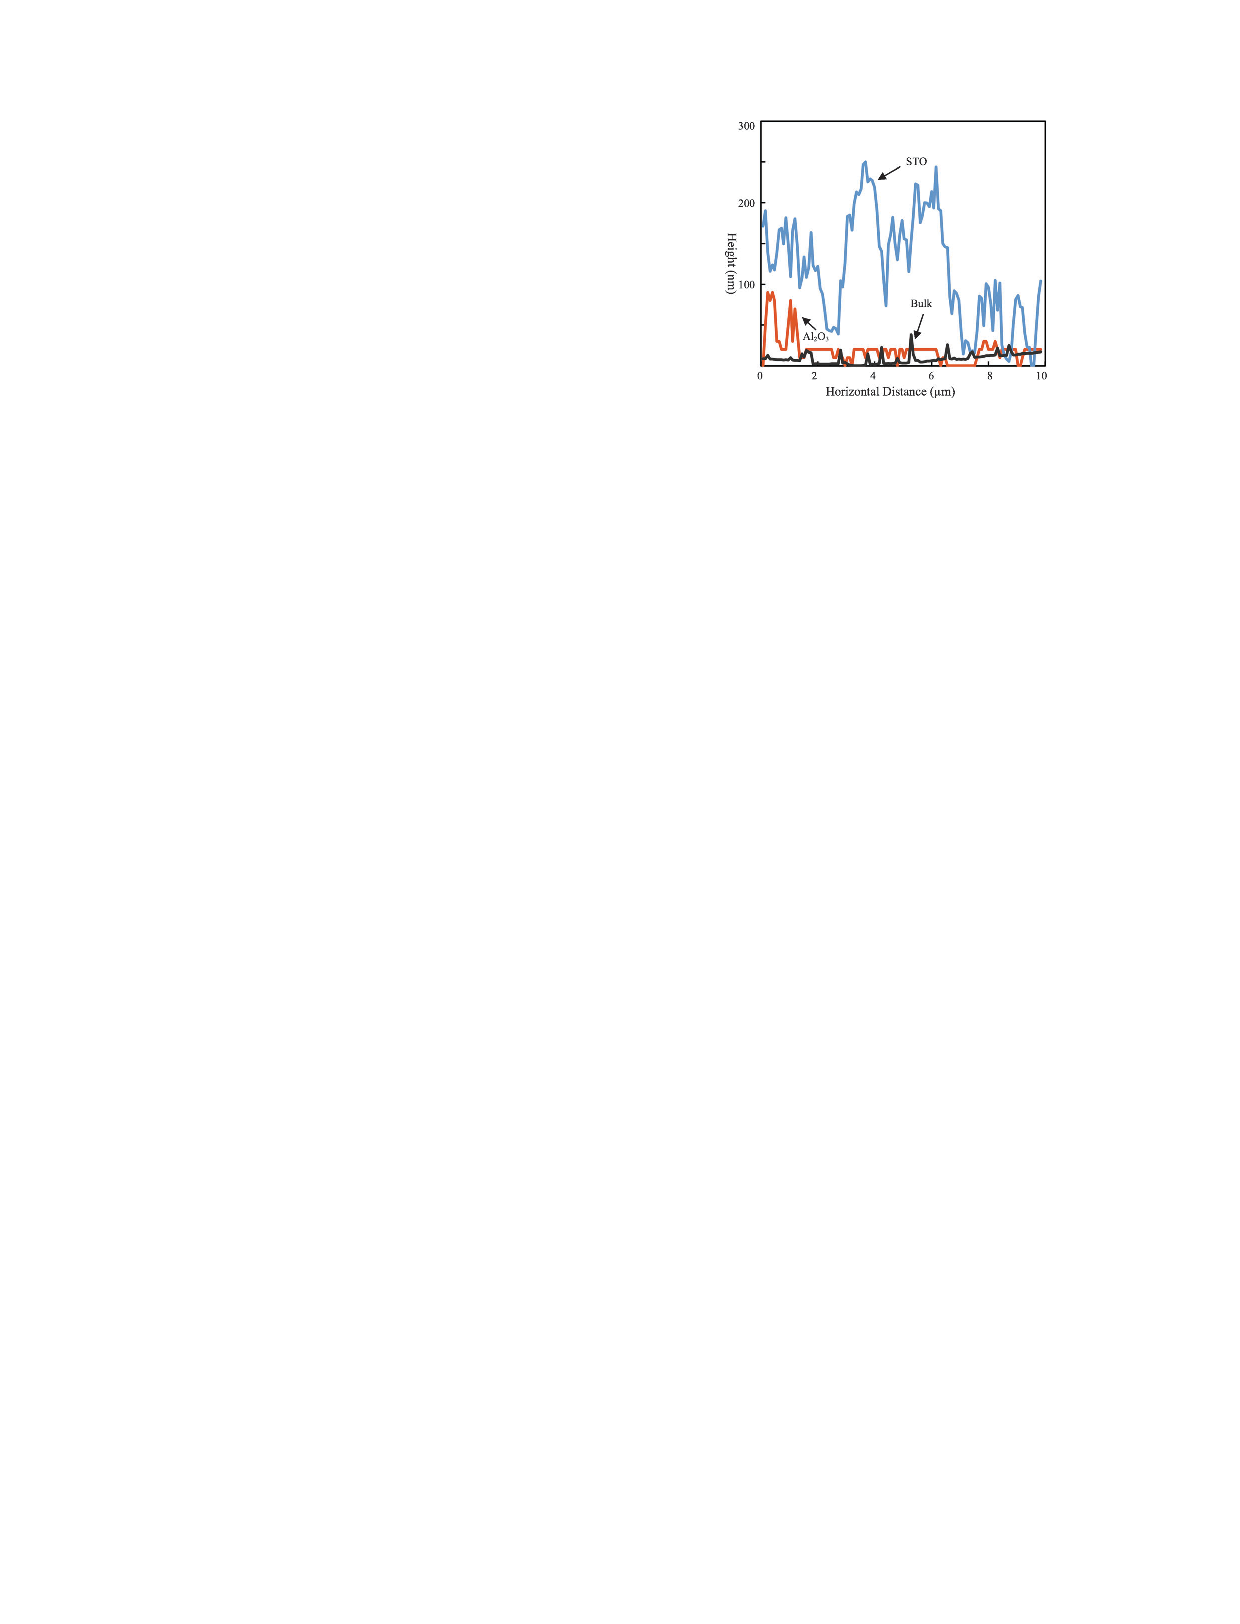
\includegraphics[width=0.8\textwidth]{lineprofiles.pdf}
\caption[Line profiles from \figureref{thinfilmresults}]{%
	Topography along lines from the \abbr{AFM} micrographs in \figureref{thinfilmresults}.

	The arrows next to the micrographs in \figureref{thinfilmresults}(d)-(f) 
	indicate the location of the horizontal line used for \figureref{lineprofiles}.}
\label{fig:lineprofiles}
\end{center}
\end{figure}
%\sidefigure[Line profiles from \figureref{thinfilmresults}]{%
%	Topography along lines from the \abbr{AFM} micrographs in
\figureref{thinfilmresults}. 
%	The arrows next to the micrographs in \figureref{thinfilmresults}(d)-(f) 
%	indicate the location of the horizontal line used for \figureref{lineprofiles}.
%	\label{fig:lineprofiles}
%	}{%
%	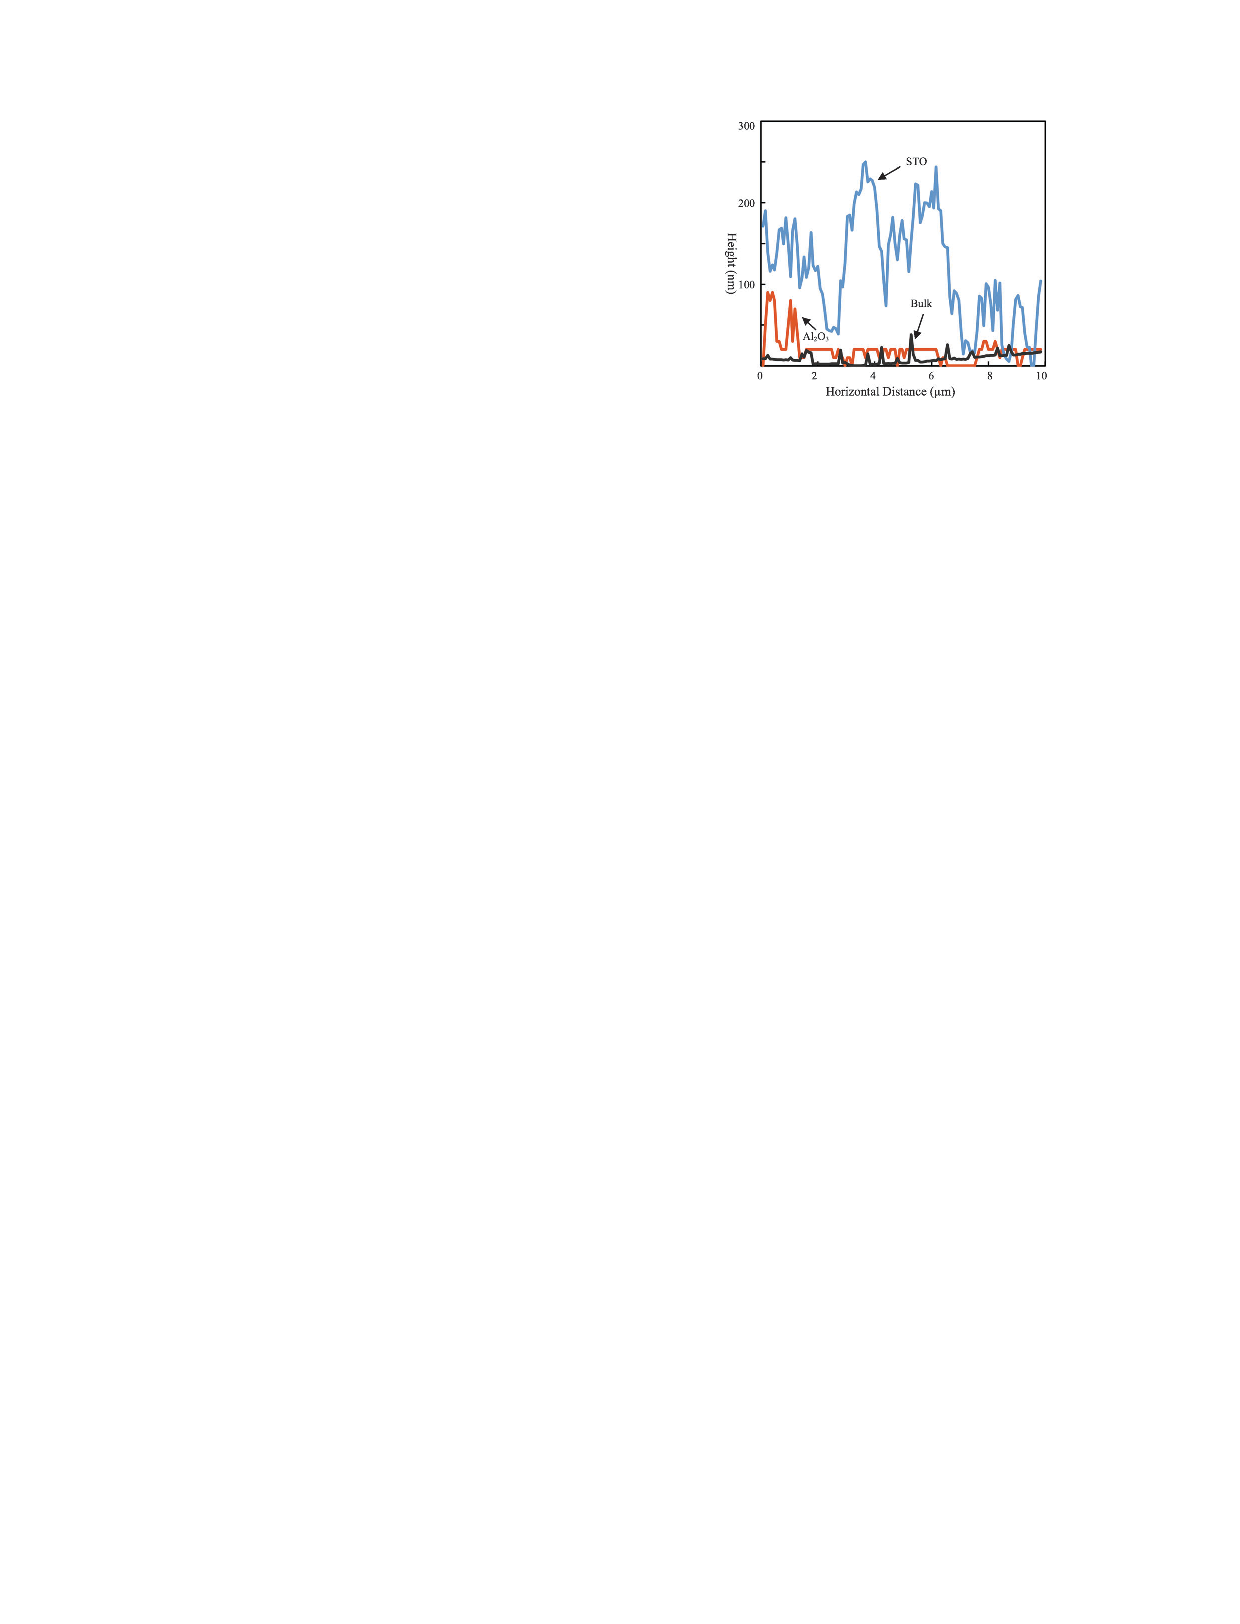
\includegraphics[width=\marginparwidth]{lineprofiles.pdf}
%}{0}
The differences in the heights of the Ag on the three surfaces are shown quantitatively in
\figureref{lineprofiles}, which compares the topography along lines from the three
micrographs in \figureref{thinfilmresults}(d)-(f). The heights of the Ag deposits on the
\textalpha-\ce{Fe2O3}/\ce{SrTiO3}(111) heterostructure range from 100 to
\SI{250}{\nano\meter}.  On the other two surfaces, all of the deposits are less than
\SI{100}{\nano\meter}.  The images in \figureref{thinfilmresults} are characteristic of
all areas that were examined.

The results presented in this chapter were consistently observed over multiple samples. In
all cases, the film on \ce{SrTiO3}(111) was significantly more reactive than the film on
alumina. The reactivity difference was so extreme that it could be used to visually
distinguish the films after reaction. After longer reaction times (on the scale of minutes
to an hour), the entire surface of the film supported on \ce{SrTiO3}(111) was covered with
silver reaction product, and excess silver was visible floating in the reaction solution.
On the film on alumina after the same reaction time, little to no reaction product could
be observed with the naked eye.


\section{Discussion}
\label{sec:single.crystal.discussion}


The results presented in \figureref{thinfilmresults} and \figureref{lineprofiles}
demonstrate that the \textalpha-\ce{Fe2O3} film on \ce{SrTiO3}(111) has a much higher
photochemical reactivity for the reduction of silver ions than a comparable film on
\ce{Al2O3} and even bulk hematite.  The images in \figureref{thinfilmresults} reveal that
the film on \ce{SrTiO3} has the greatest silver surface coverage. The data in
\figureref{lineprofiles} show that the silver deposits are larger for films on \ce{SrTiO3}
than for films on alumina or for bulk \ce{Fe2O3}. 

This result is surprising for multiple reasons.  The structure of both films does not vary
enough to cause the marked difference in reactivity. Both films are (0001)-oriented
\textalpha-\ce{Fe2O3} of nominally equal thickness.  \abbr{AFM} scans show that the
morphology of the films is similar. The thickness of the films used in this experiment was
\texttildelow\SI{50}{\nano\meter}. Based solely on the depth of light absorption in
\ce{Fe2O3}, one could expect the bulk sample to be much more reactive than the films.  The
penetration depth of \SI{470}{\nano\meter} photons in hematite reported to be
approximately \SI{450}{\nano\meter}.\cite{Marusak:1980gc}  The films were of a sufficient
thickness to absorb only a fraction of the incident light, in contrast to the bulk sample,
which was much thicker than the absorption depth. Furthermore, based on the index of
refraction mismatch, the \ce{Al2O3}/\ce{Fe2O3} interface is more reflective than the
\ce{SrTiO3}/\ce{Fe2O3} interface, so internal reflection leading to an increase in path
length in the film cannot account for the difference in reactivity.  In both cases, the
band gap of the substrate (> \SI{8}{\electronvolt} for \ce{Al2O3},\cite{French:1998wj} and
\SI{3.2}{\electronvolt}  for \ce{SrTiO3}\cite{Cardona:1965vw}) is too large for the light
used in this experiment to generate a significant number of electron-hole pairs.  We can
therefore conclude that the majority of the electron hole pairs were generated in the
films. Neither substrate was able to participate in photochemical reactions by absorbing
light and shuttling generated charge carriers to the surface of the film, as seen in
previous experiments with UV light and \ce{TiO2}/\ce{BaTiO3}
heterostructures.\cite{Burbure:2010ti,Burbure:2010go}  Despite the fact that it absorbs
less light, the film supported by \ce{SrTiO3} was more reactive than the bulk sample.

One possible explanation for the increased reactivity of the film supported on \ce{SrTiO3}
lies in the band structure of the substrate materials. Previous authors investigating the
\ce{SrTiO3}/\ce{Fe2O3} system have suggested that the \ce{Fe2O3} layer acts as an electron
acceptor transferring holes to the active \ce{SrTiO3} photoanode.\cite{Wang:2007fp} If
\ce{Fe2O3} acts as a sink for electrons at the back of the active layer, more holes can
reach the surface without recombining.  One could make the reverse argument here to
explain the current observations.  In this case, the \ce{SrTiO3} layer can act as a hole
acceptor, increasing the number of photogenerated electrons that reach the \ce{Fe2O3}
surface to participate in the photocathodic reaction.  This could explain why the thin
film sample has a much higher reactivity than the bulk material, even though less light is
absorbed.  Because the band gap of alumina is significantly larger than that of the
\ce{Fe2O3} film, there exists a significant barrier to charge transfer across the
interface.  As a result, the alumina substrate cannot accept holes, and the recombination
rate within the film is not decreased.

Assuming \ce{SrTiO3} acts as a hole acceptor and this is responsible for the increased
reactivity, we must also consider what happens to these holes.  In our experimental
set-up, there is no path to ground or to complete the circuit with the solution.  If the
holes were to build up in the substrate, the heterostructure would become charged and the
reaction would stop.

A second explanation is that uncompensated charge at the \ce{SrTiO3}(111) acts to separate
electrons and holes, reducing recombination.  The individual (111) atomic planes in the
\ce{SrTiO3} structure have alternate positive (\ce{Ti^{4+}}) and negative charges
(\ce{SrO3^{4-}}).  Terminating the surface in a single charge is energetically costly, so
the surface breaks up into positive domains with Ti termination and negative domains with
\ce{SrO3} termination.  Giocondi\cite{Giocondi:2003wc} has shown that the oppositely
charge surface domains have different photochemical properties, with one favoring
reduction and the other favoring oxidation.  Note that \textalpha-\ce{Fe2O3} also has
planes of alternating charge parallel to the interfaces plane.  However, the trivalent
charges of the (0001) planes cannot completely compensate the charge from the
\ce{SrTiO3}(111) surface.  These charges can, however, exactly compensate the charges on
the isostructural, isoelectronic \ce{Al2O3}(0001) surface.
\begin{figure}
\begin{center}
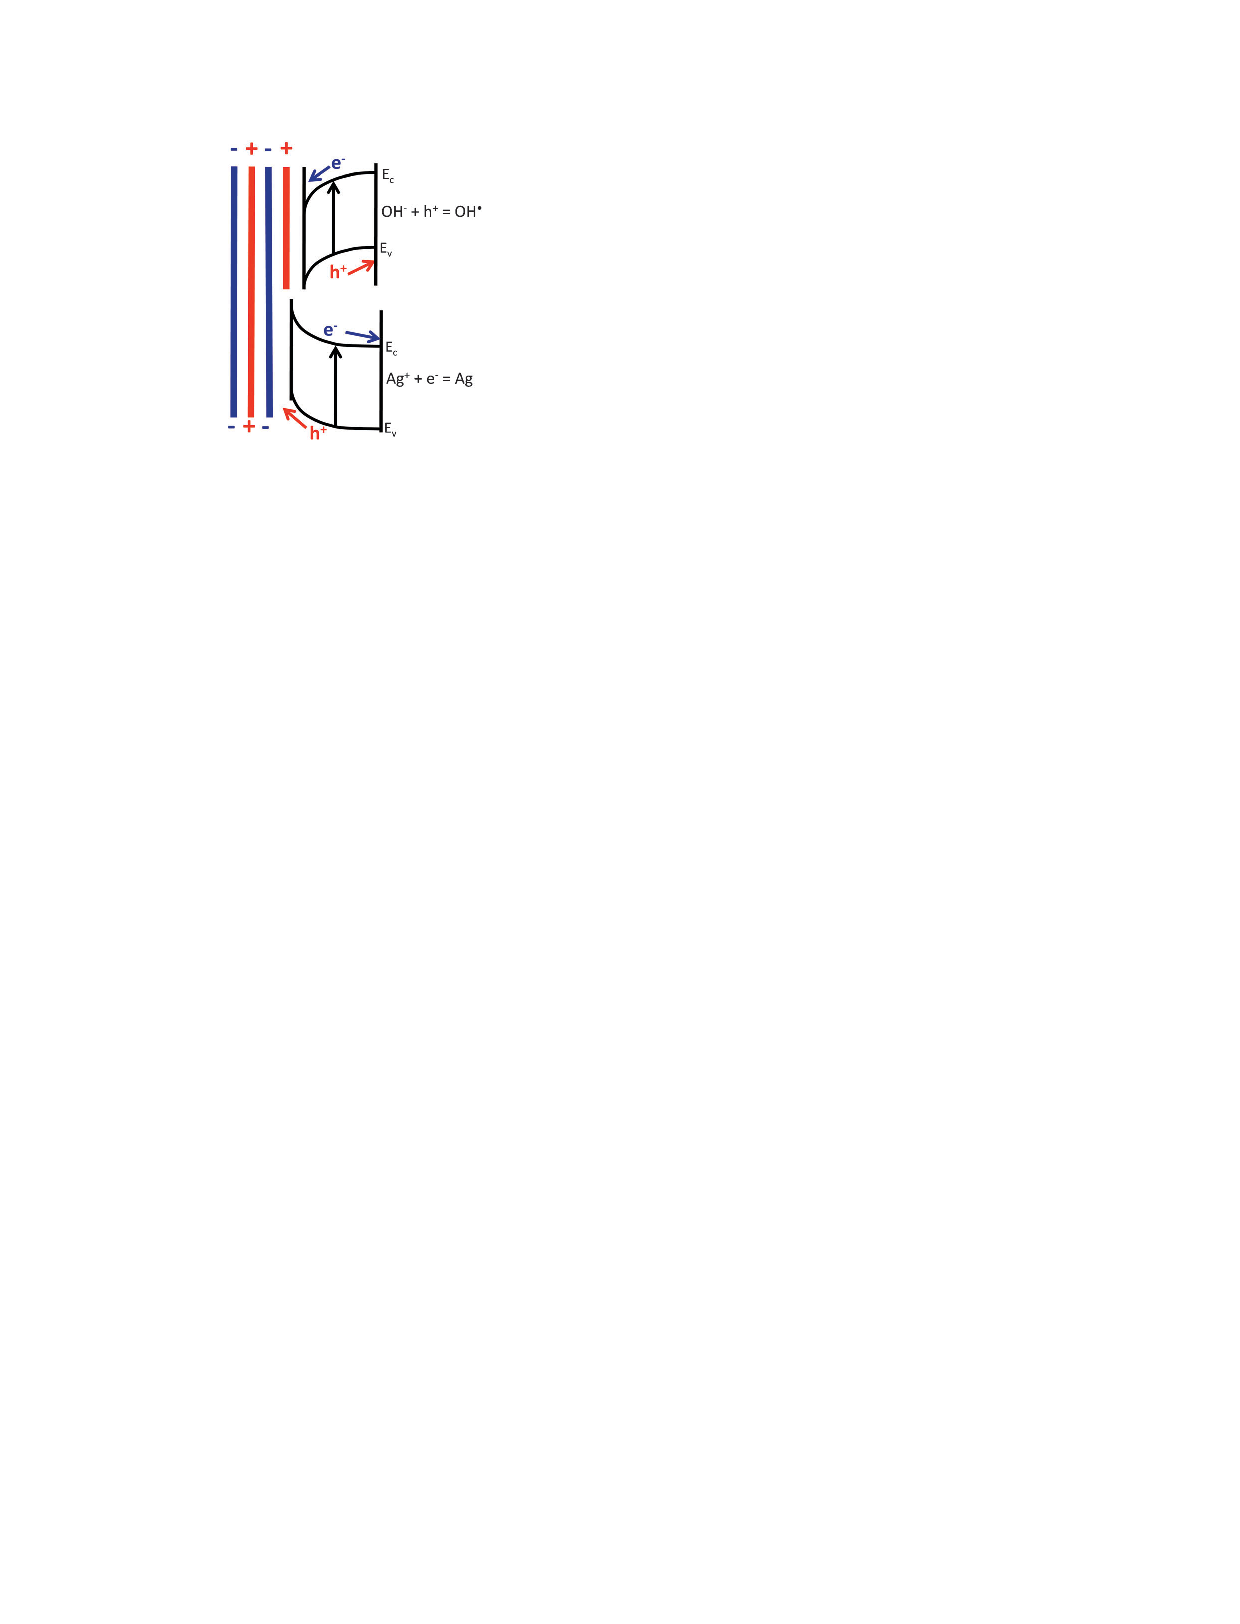
\includegraphics[width=0.6\textwidth]{polarterms.pdf}
\caption[Charges at internal interface between \ce{SrTiO3} and \ce{Fe2O3}]{%
		Schematic depiction of the charges at the internal interface 
		between \ce{SrTiO3}(111) and \textalpha-\ce{Fe2O3}. There are 
		alternating planes of charge along the [111] direction and some 
		areas are positively terminated (upper) and others have a negative 
		termination (lower). The charged termination will cause the bands 
		in the film to bend in a way that will move carriers in opposite 
		direction. E$_C$ and E$_V$ label the conduction and valence band 
		edges, respectively.}
\label{fig:polarterms}
\end{center}
\end{figure}
%\sidefigure[Charges at internal interface between \ce{SrTiO3} and \ce{Fe2O3}]{%
%		Schematic depiction of the charges at the internal interface 
%		between \ce{SrTiO3}(111) and \textalpha-\ce{Fe2O3}. There are 
%		alternating planes of charge along the [111] direction and some 
%		areas are positively terminated (upper) and others have a negative 
%		termination (lower). The charged termination will cause the bands 
%		in the film to bend in a way that will move carriers in opposite 
%		direction. E$_C$ and E$_V$ label the conduction and valence band 
%		edges, respectively.
%	\label{fig:polarterms}
%	}{%
%	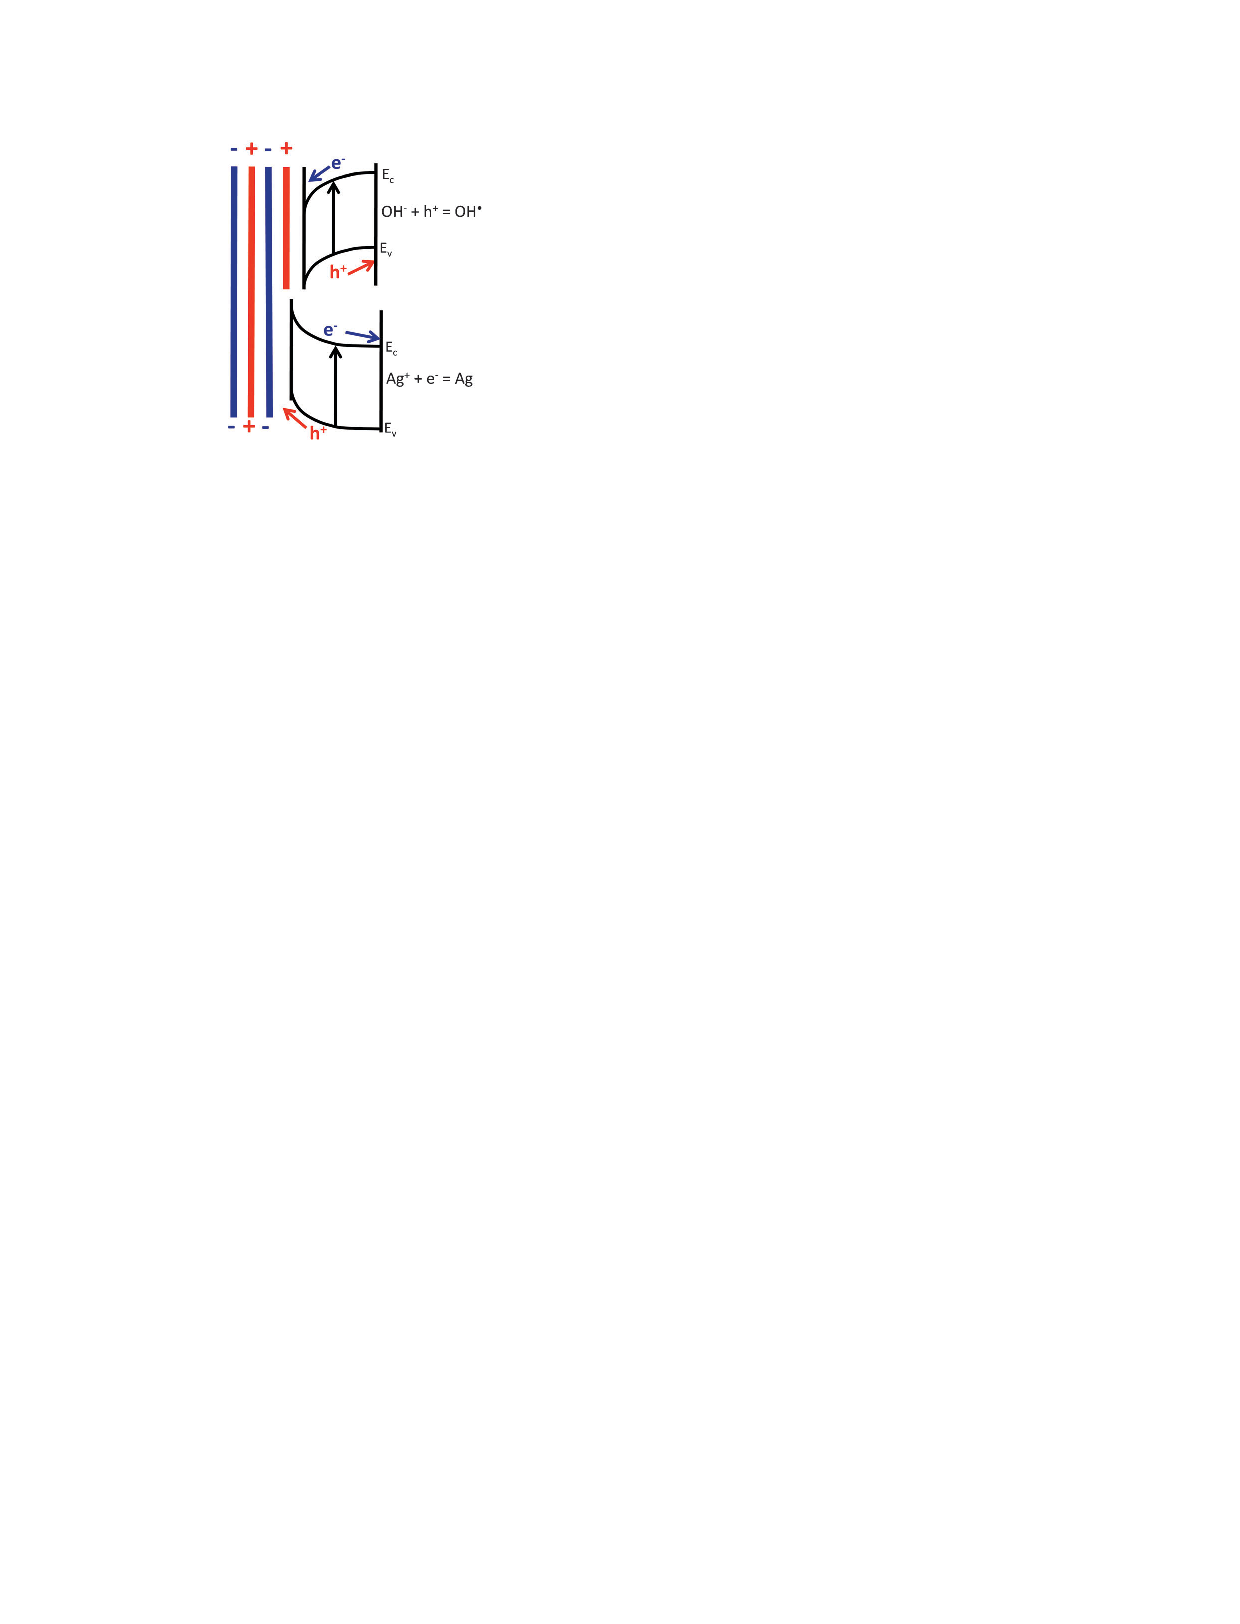
\includegraphics[width=\marginparwidth]{polarterms.pdf}
%}{-4}
\figureref{polarterms} illustrates a schematic view of our proposed explanation for the
enhanced reactivity of \textalpha-\ce{Fe2O3}/\ce{SrTiO3}(111) heterostructures. In the
hematite film above positively terminated domains, bands bend downward and draw
photogenerated electrons to the internal interface while holes are drawn to the
hematite/solution interface.  The opposite occurs in negative domains and this is where
the reduction of silver occurs.  In each case, the complementary carriers can recombine
within \ce{SrTiO3}, so there is no charge accumulation.  Note that the previous work
showed that charged domains on the \ce{SrTiO3}(111) surface have dimensions on the order
1-2~\si{\micro\meter} (refer to \figureref{giocondi}).  This may account for the highly
heterogeneous distribution of Ag on the surface of the heterostructure in
\figureref{thinfilmresults}(e).

Finally, it is noted that the lattice parameter mismatch is significantly larger for 
films on alumina than films on \ce{SrTiO3}. The mismatch between the 
a-axis lattice parameter for \ce{Fe2O3} and the atomic spacing of 
(111)-\ce{SrTiO3} is 3.2\%. The mismatch between alumina and hematite is 
\texttildelow{}20\%. As a result, the films on alumina are expected to 
have a much higher defect concentration than films on \ce{SrTiO3}. 
Defects are known to act as recombination sites for charge carriers. 
The higher concentration of defects in the film on alumina could help 
explain the low activity of this film.


\section{Conclusions}
\label{sec:single.crystal.conclusions}


In summary, \ce{Fe2O3} films on \ce{SrTiO3} substrates show greatly enhanced reactivity
when compared to films on \ce{Al2O3} substrates. The reactivities of \ce{SrTiO3} supported
films are also greater than the reactivity of bulk \ce{Fe2O3} samples.  The results show
that the visible light photochemical activity of hematite, \textalpha-\ce{Fe2O3}, can be
enhanced through the proper choice of substrate material. If polar terminations of the
\ce{SrTiO3}(111) surface are responsible for the increased reactivity, then the enhanced
reactivity of the heterostructure should not occur on nonpolar substrate orientations. 
For example, the \ce{SrTiO3}(100) surface is nonpolar and does not have charged domains or
spatially selective reactivity.\cite{Giocondi:2003wc} Results of photochemical activity of
\ce{Fe2O3} films on polycrystalline perovskite substrates are included later in this
document.